\documentclass[dissertation.tex]{subfiles} 
\begin{document}

\chapter{Motivation for Physics Beyond the Standard Model}
\label{chap:Motivation for Physics Beyond the Standard Model}

In the 1960s, Sheldon Glashow, Steven Weinberg, and Abdus Salam proposed a mathematical framework that unified the electromagnetic and weak forces at an energy scale in the hundreds of GeV/c, as well as a mechanism for breaking the electroweak symmetry at low energies \cite{Glashow_Weinberg_and_Salam}.  At the same time, Murray Gell-Mann introduced the concept of quarks to describe hadron spectroscopy, a concept that would later grow into quantum chromodynamics (QCD), the full theory of the strong force \cite{Gell-Mann}.  These two key developments motivated the unified representation of particle physics as a set of fields whose dynamics are invariant under the Standard Model (SM) gauge group

\begin{equation}
SU(3)_{C} \otimes SU(2)_{L} \otimes U(1)_{Y}
\end{equation}
%
where $SU(3)_{C}$ describes the quark QCD interactions, $SU(2)_{L}$ describes the weak interactions among quarks and leptons, and $U(1)_{Y}$ describes the electromagnetic interaction.

The Standard Model has been an extremely successful predictor of particle production and interaction cross-sections and decay rates, as well as of the exact masses of the electroweak force carriers.  The case for the validity of the Standard Model was bolstered by the many precision QCD and electroweak measurements carried out at the Large Electron-Positron (LEP) collider, which ran from 1989-2000 at center-of-mass energies between 65 and 104 GeV/c \cite{Drees}.  Figure~\ref{fig:LEP} shows some of the highlights of the LEP program.

\begin{figure}
	\centering
	\subfloat[Total hadronic cross-section as a function of collider center-of-mass energy.]{\label{fig:LEP_hadronic_xsec}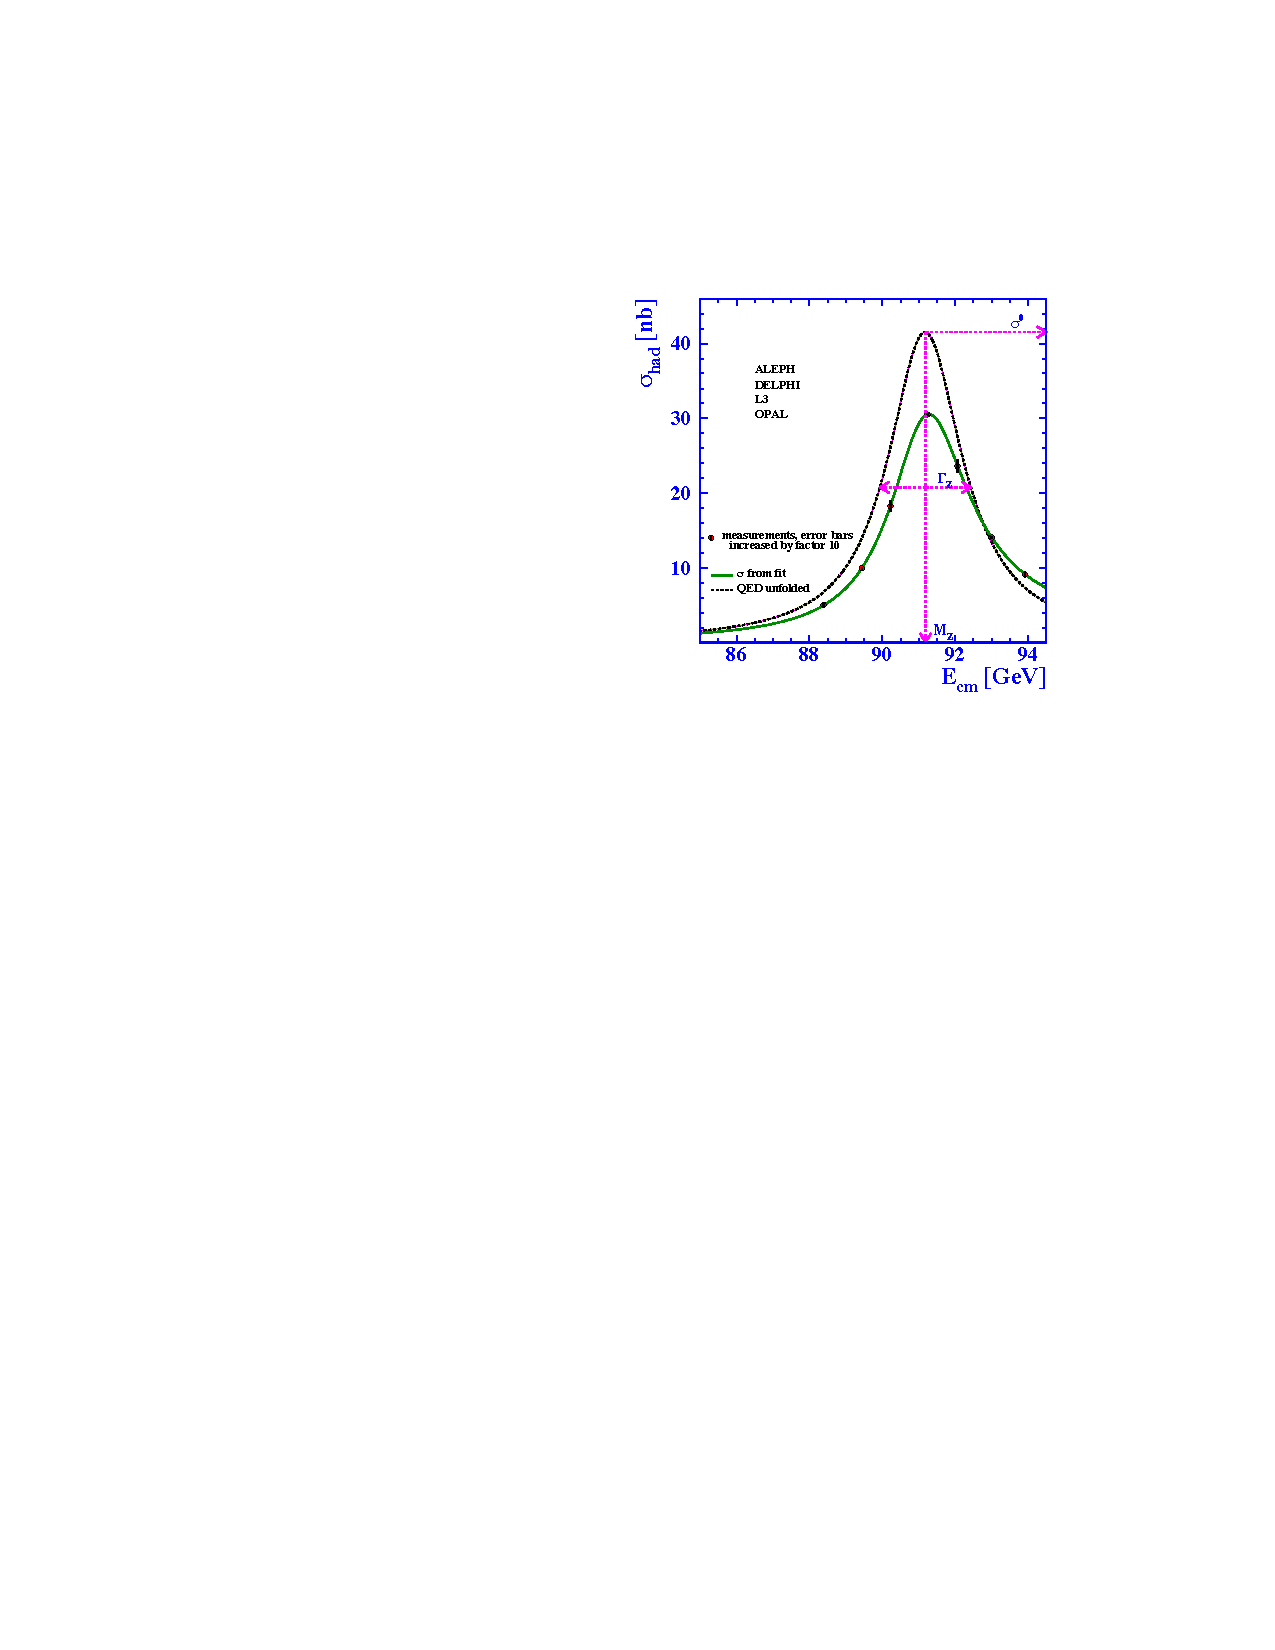
\includegraphics[scale=0.7]{LEP_hadronic_xsec}}
	\hspace{1cm}
	\subfloat[Measured and predicted dependence of the $q\overline{q}$, $\mu^{+}\mu^{-}$, and $\tau^{+}\tau^{-}$ pair production cross sections on LEP center-of-mass energy.]{\label{fig:LEP_pair_production_xsecs}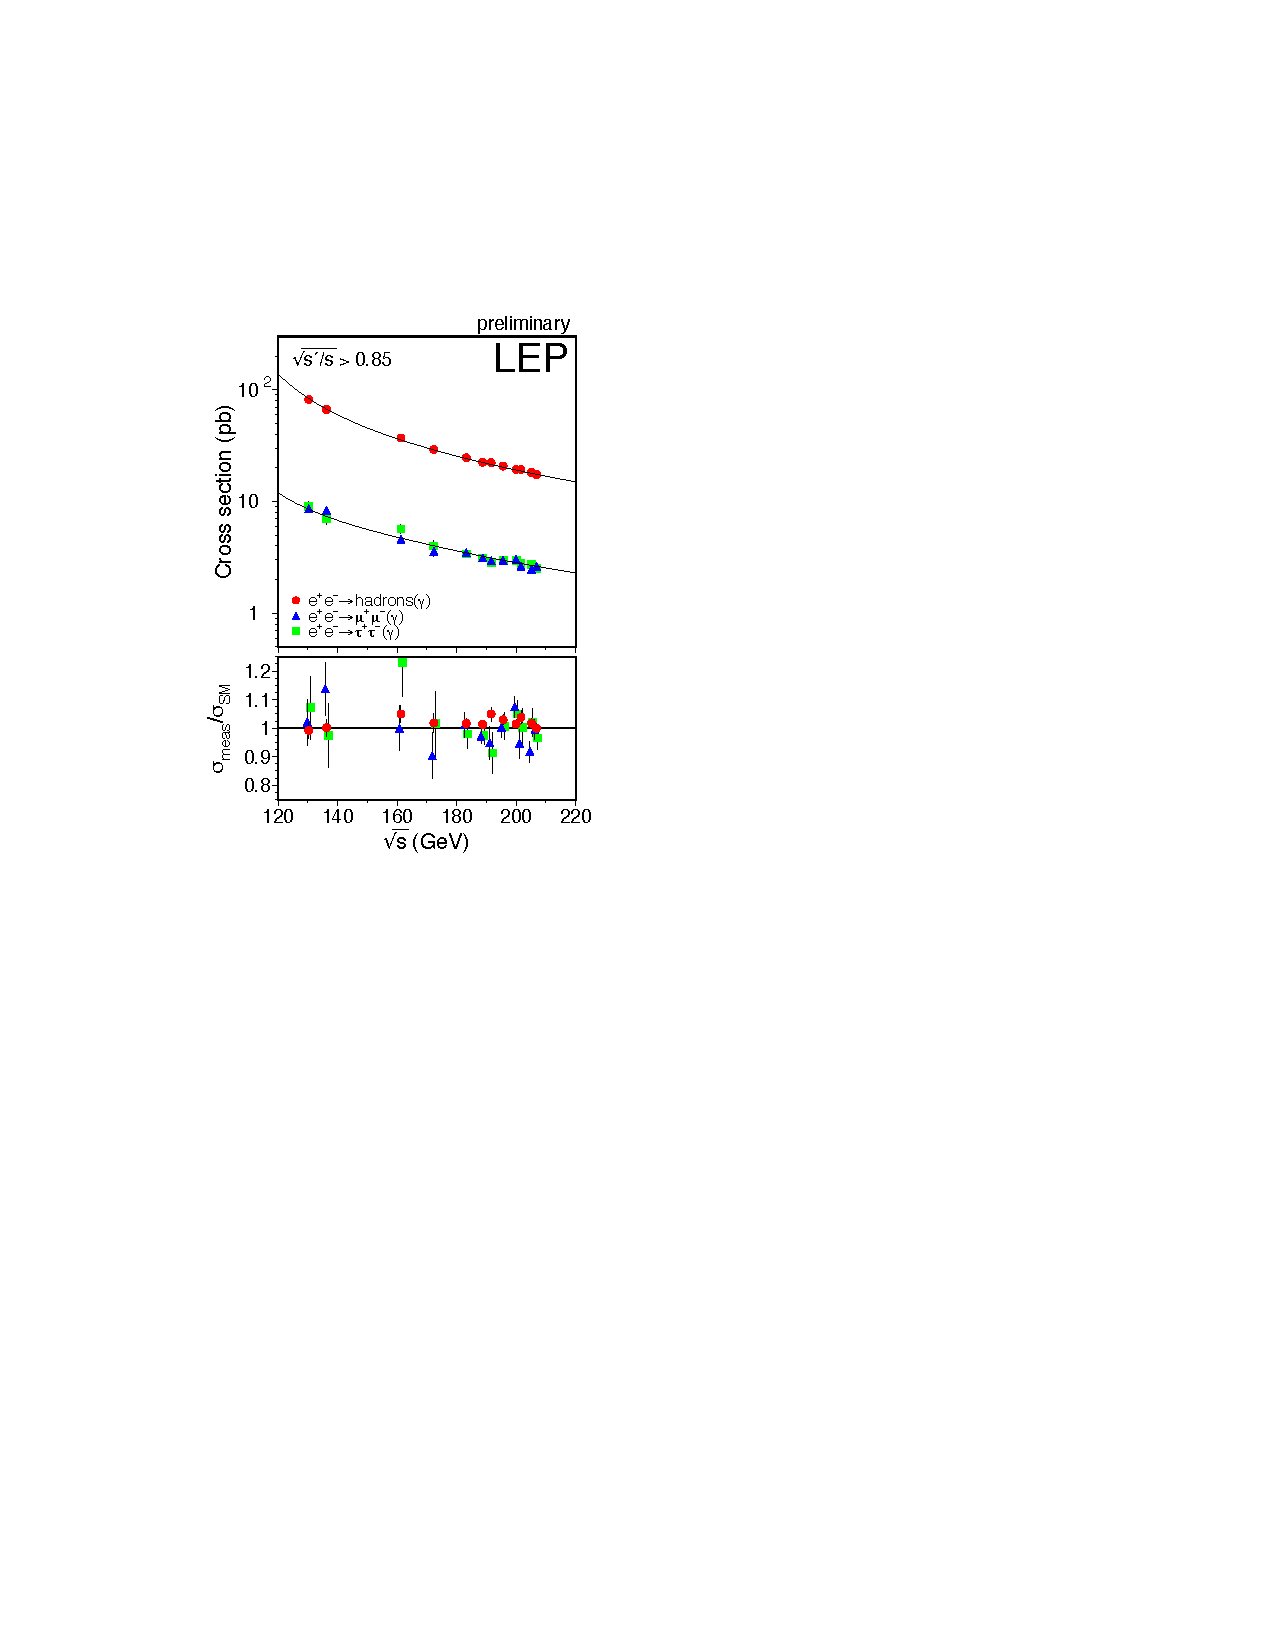
\includegraphics[scale=0.7]{LEP_pair_production_xsecs}}
	\\
	\subfloat[Measured and predicted dependence of the $W^{+}W^{-}$ pair production cross section on LEP center-of-mass energy.]{\label{fig:LEP_W_pair_production_xsec}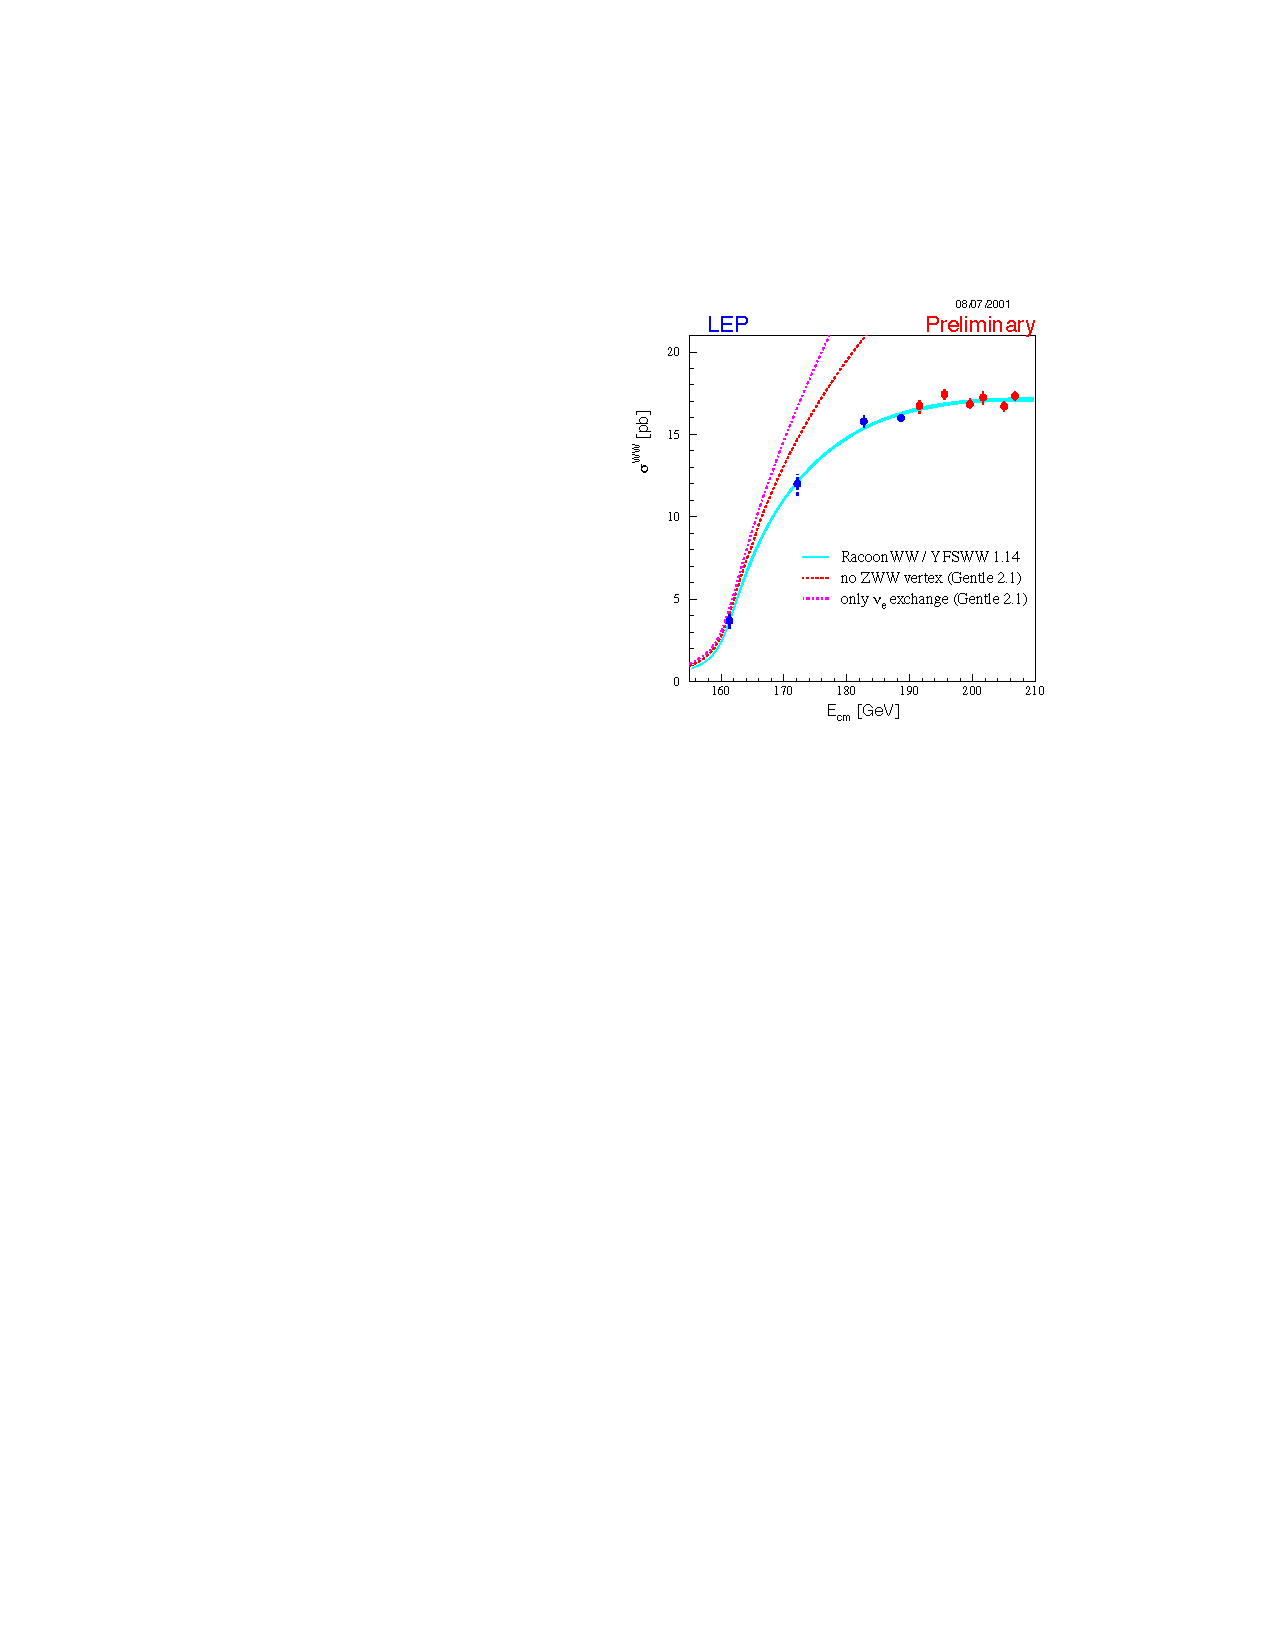
\includegraphics[scale=0.7]{LEP_W_pair_production_xsec}}
	\hspace{1cm}
	\subfloat[Measured and predicted dependence of the strong coupling constant $\alpha_{s}$ on LEP center-of-mass energy.]{\label{fig:LEP_alphaS_running}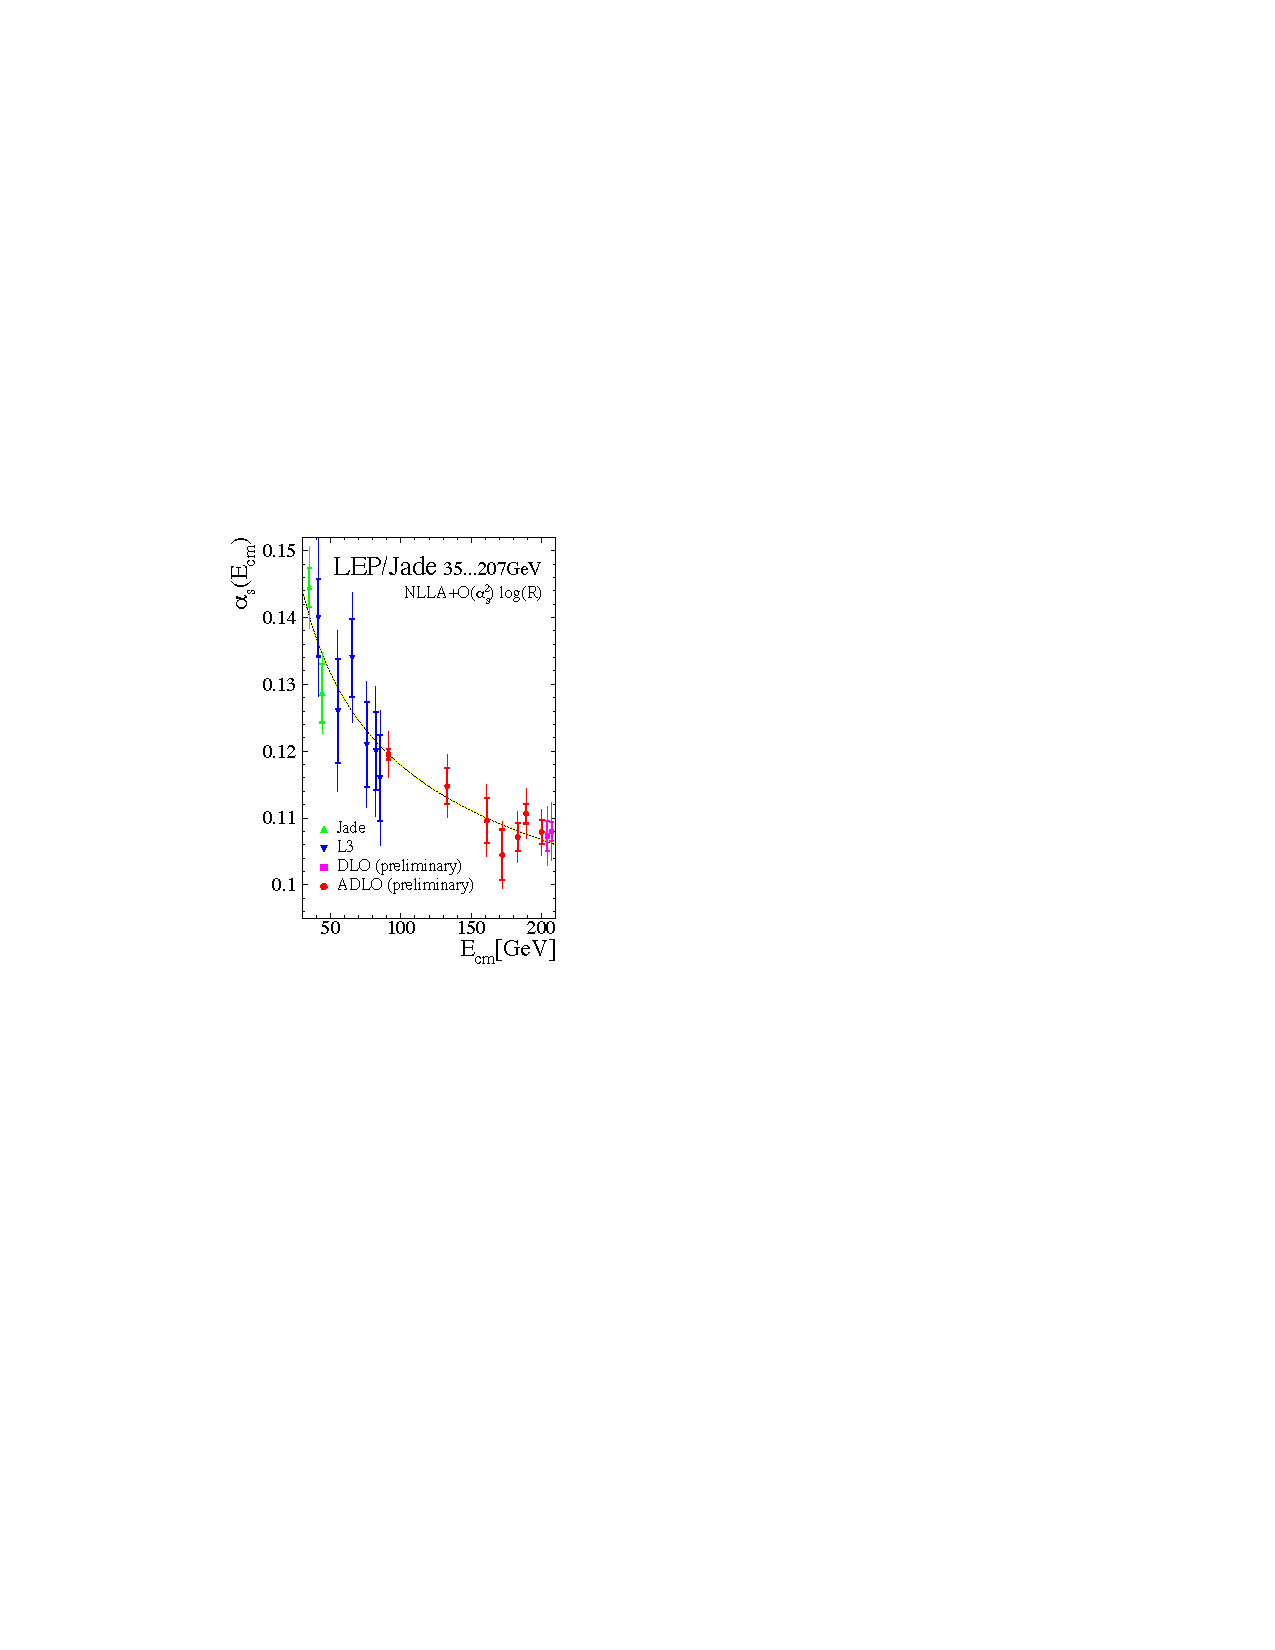
\includegraphics[scale=0.7]{LEP_alphaS_running}}
	\caption{Selected LEP measurements demonstrating its contribution to the precise understanding of the Standard Model.  Reprinted from \cite{Drees}.}
	\label{fig:LEP}
\end{figure}

However, there are still deep theoretical problems with the Standard Model, stemming from the introduction of the Higgs scalar into the theory to break electroweak symmetry \cite{Higgs}.  Since the Higgs self-energy diagram is quadratically sensitive to the ultraviolet cutoff scale, and assuming that there are no new important energy scales of physics between the weak scale ($\mathcal{O}$($10^{2}$ GeV/c)) and the Planck scale ($\mathcal{O}$($10^{19}$ GeV/c)), in order to be consistent with experimental measurements, this diagram must include a remarkable 17-orders-of-magnitude cancellation that is otherwise poorly motivated \cite{Aitchison}.  The quest to find new physics at an intermediate energy scale between the weak and Planck scales, and thus extend the Standard Model, was the driving force behind the construction of the Large Hadron Collider (LHC) in 2009, the world's highest energy particle accelerator to date.

In this chapter I will briefly describe the Standard Model and electroweak symmetry breaking (EWSB) and the problems that the Standard Model is as yet ill-prepared to address.

\section{The Standard Model and Electroweak Symmetry Breaking}
\label{sec:The Standard Model and Electroweak Symmetry Breaking}

All of the elementary matter particles (fermions)---quarks, charged leptons, and neutrinos---can be put in fundamental representations of the SM gauge groups.  The fermion content of the Standard Model is summarized in Table~\ref{tab:SM_particle_summary}.  The left-handed doublets are analogous to the spinors of non-relativistic quantum mechanics, with the $z$ component of ``weak isospin" $I_{3}$ equal to +1/2(-1/2) for the upper(lower) component of the doublet.

\begin{table}[htbp]
\caption{Fermion content of the Standard Model.  Adapted from ref. \cite{FNAL_SM_particle_table}.}
\begin{tabular}{|l|c|m{5.5cm}|c|}
\hline
\multicolumn{1}{|c|}{Type} & Notation & Representation under $SU(3)_{C} \otimes SU(2)_{L} \otimes U(1)_{Y}$ & Couples to \\
\hline
\hline
\multirow{5}{*}{\begin{tabular}{@{}l@{}}Left-handed\\quark doublet\end{tabular}} & $\left(\begin{array}{c}u_{L} \\d_{L}\end{array}\right)$ & \multicolumn{1}{c|}{\multirow{5}{*}{($\mathbf{3}$, $\mathbf{2}$, $\frac{1}{6}$)}} & \multirow{5}{*}{$g$, $W$, $\gamma$} \\
 & $\left(\begin{array}{c}c_{L} \\s_{L}\end{array}\right)$ & & \\
 & $\left(\begin{array}{c}b_{L} \\t_{L}\end{array}\right)$ & & \\
\hline
\multirow{3}{*}{\begin{tabular}{@{}l@{}}Right-handed\\up-type quark singlet\end{tabular}} & $u_{R}^{\dagger}$ & \multicolumn{1}{c|}{\multirow{3}{*}{($\mathbf{\bar{3}}$, $\mathbf{1}$, -$\frac{2}{3}$)}} & \multirow{3}{*}{$g$, $W$, $Z$, $\gamma$} \\
 & $c_{R}^{\dagger}$ & & \\
 & $b_{R}^{\dagger}$ & & \\
\hline
\multirow{3}{*}{\begin{tabular}{@{}l@{}}Right-handed\\down-type quark singlet\end{tabular}} & $d_{R}^{\dagger}$ & \multicolumn{1}{c|}{\multirow{3}{*}{($\mathbf{\bar{3}}$, $\mathbf{1}$, $\frac{1}{3}$)}} & \multirow{3}{*}{$g$, $W$, $Z$, $\gamma$} \\
 & $s_{R}^{\dagger}$ & & \\
 & $t_{R}^{\dagger}$ & & \\
\hline
\multirow{5}{*}{\begin{tabular}{@{}l@{}}Left-handed\\lepton doublet\end{tabular}} & $\left(\begin{array}{c}\bar{\nu}_{eL} \\e_{L}\end{array}\right)$ & \multicolumn{1}{c|}{\multirow{5}{*}{($\mathbf{1}$, $\mathbf{2}$, -$\frac{1}{2}$)}} & \multirow{5}{*}{$W$, $\gamma$} \\
 & $\left(\begin{array}{c}\bar{\nu}_{\mu L} \\\mu_{L}\end{array}\right)$ & & \\
 & $\left(\begin{array}{c}\bar{\nu}_{\tau L} \\\tau_{L}\end{array}\right)$ & & \\
\hline
\multirow{3}{*}{\begin{tabular}{@{}l@{}}Right-handed\\charged lepton singlet\end{tabular}} & $e_{R}^{\dagger}$ & \multicolumn{1}{c|}{\multirow{3}{*}{($\mathbf{\bar{1}}$, $\mathbf{1}$, 1)}} & \multirow{3}{*}{$W$, $Z$, $\gamma$} \\
 & $\mu_{R}^{\dagger}$ & & \\
 & $\tau_{R}^{\dagger}$ & & \\
\hline
\end{tabular}
\label{tab:SM_particle_summary}
\end{table}

There are two types of weak interactions: flavor-changing charged currents, in which an up-type and down-type quark or charged lepton and neutrino couple to a charged $W$, and neutral currents, in which a fermion couples to another of the same flavor and to a neutral $Z$.  The charged current interaction is maximally parity violating---it only couples left-handed fermion doublets.  The neutral current interaction has a term coupling left-handed doublets and a term coupling right-handed singlets.  There are no mass terms of the form $m_{f}^{2}(f_{L}\bar{f}_{R} + f_{R}\bar{f}_{L})$ in the electroweak part of the Lagrangian, as these would violate gauge invariance \cite{Quigg}.  The simplest way to link the left-handed and right-handed fermions is via a Yukawa interaction $-\xi\left[\bar{f}_{R}(\phi^{\dagger}f_{L}) + (\bar{f}_{L}\phi)f_{R}\right]$ where $\phi$ is a complex doublet of scalar fields \cite{Quigg}.

The fermion interaction part of the Lagrangian is \cite{Quigg}

\begin{eqnarray}
\mathcal{L}_{\mathrm{int}} &=& \bar{f}_{R}i\gamma^{\mu}(\partial_{\mu} + i\frac{g_{Y}}{2}A_{\mu}Y)f_{R} \nonumber \\
&&+\mbox{ }\bar{f}_{L}i\gamma^{\mu}(\partial_{\mu} + i\frac{g_{Y}}{2}A_{\mu}Y + i\frac{g_{L}}{2}\overrightarrow{\tau}\cdot\overrightarrow{b}_{\mu})f_{L}
\end{eqnarray}
%
where $g_{Y}$ and $g_{L}$ are the electromagnetic and weak coupling constants, respectively; $Y$ is the weak hypercharge; $A_{\mu}$ is the EM gauge field; $\overrightarrow{b}_{\mu}$ is a three-component vector of weak gauge fields; and $\overrightarrow{\tau}$ is a three-component vector of the three Pauli matrices.  Before electroweak symmetry breaking, the three weak gauge fields and the one EM gauge field are massless.  The three weak gauge fields correspond to the three generators (the Pauli matrices) of $SU(2)_{L}$.  The one EM gauge field corresponds to the one generator (the real scalar $Y$) of $U(1)_{Y}$, where $Y = 2(Q - I_{3})$ ($Q$ is electric charge).  For the $SU(3)_{C}$ part of the Lagrangian, there are eight massless gauge fields (the gluons) corresponding to the eight generators of $SU(3)_{C}$ (the Gell-Mann matrices).

To break the electroweak symmetry implicit in the massless gauge bosons, a doublet of complex scalar fields (the Higgs) is introduced.  It has a potential \cite{Quigg}

\begin{eqnarray}
V(\phi^{\dagger}\phi) &=& \mu^{2}\phi^{\dagger}\phi + |\lambda|(\phi^{\dagger}\phi)^{2}.
\end{eqnarray}

Since $\mu^{2} < 0$, the potential has the shape of a sombrero, as shown in Figure~\ref{fig:Higgs_potential}.  At the minimum of the potential, the scalar fields are not zero, but have some positive vacuum expectation value (VEV) (it can be chosen such that one component is zero and the other is $\sqrt{-\mu^{2}/2|\lambda|}$).  Nature spontaneously chooses one of the infinitely many vacua along the circle of minimum $V$ in ($\Re\left[\phi\right]$, $\Im\left[\phi\right]$) space.

\begin{figure}
	\centering
	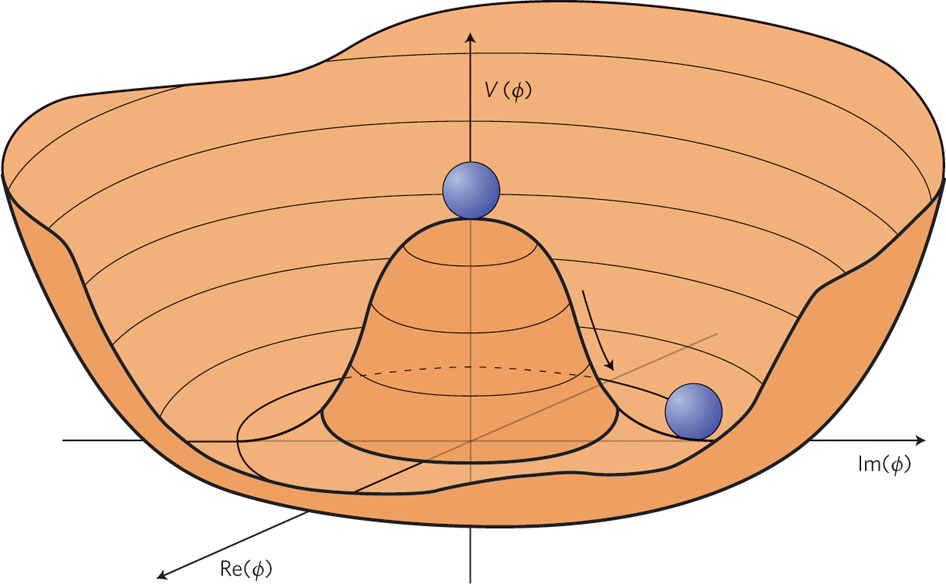
\includegraphics[scale=0.3]{Higgs_potential}
	\caption{Higgs potential (the sombrero) as a function of the real and imaginary parts of the complex scalar field.  The movement of the balls shows that the symmetry $\phi = 0$ is spontaneously broken, the stable vacuum state of nature being somewhere along the circle of minimum potential.  Reprinted from Fig. 1 of ref. \cite{Alvarez-Gaume}.}
	\label{fig:Higgs_potential}
\end{figure}

Expanding $\phi$ about its VEV $v$ in the Lagrangian introduces one massive scalar, the Higgs, and new mass terms for the gauge bosons.  However, the terms with positive mass are not the original $b_{1}$, $b_{2}$, $b_{3}$, and $A$ (spacetime indices dropped), but the observable $W^{\pm}$ and $Z^{0}$.  The $W^{\pm}$ are linear combinations of $b_{1}$ and $b_{2}$.  The $Z^{0}$ is one of the linear combinations of $b_{3}$ and $A$, the other being the massless photon $\gamma$.  After electroweak symmetry breaking (EWSB), the only remaining symmetry of the vacuum is electric charge, because the value of the electric charge operator acting on the Higgs VEV is zero.  As expected, there is one massless photon in the SM to reflect this symmetry.  The SM fermions can also acquire masses as a by-product of the Higgs mechanism via Yukawa terms.

\section{Problems of the Standard Model}
\label{sec:Problems of the Standard Model}

Before the formulation of the Higgs mechanism, physicists suspected that a heavy boson mediated the weak force from observations of $\beta$ decay, but had no way of putting a mass term into the Lagrangian without breaking gauge symmetry.  The Higgs mechanism of EWSB provided a way to generate masses for the $SU(2)_{L}$ gauge bosons.  Furthermore, it predicted the $W$ and $Z$ masses in terms of $g_{L}$, $g_{Y}$, and $v$.  $g_{L}$ and $g_{Y}$ could be measured in scattering experiments, and in 1983 the $W$ and $Z$ were first observed at the Super Proton-Antiproton Synchrotron (Sp$\bar{\mbox{p}}$S) at the European Organization for Nuclear Research (CERN) in Geneva, Switzerland \cite{UA1_W, UA1_Z}.  Crucially, the values of the coupling constants and the gauge boson masses predict that the Higgs VEV should be 246 GeV, so the Higgs mass should not be too much different than that if $\lambda$ is to remain small enough to do perturbation theory \cite{Gunion}.

The Higgs mechanism raises some interesting questions.
%where is the Higgs?
%- why is mu^2 negative
%- hierarchy problem
%- mass hierarchy

%show how susy solved heierarchy prob
%show how SUSY makes mu^2 negative
%show how SUSY unifies the coupling constants
%dark matter

%- tie in current Higgs hints?

\end{document}